%!TEX root = ms.tex
\beginsupplement
\appendix
\pagenumbering{arabic}
\begin{center}
\textbf{\large Supplementary Materials \\
On the Use of Information Criteria for Subset Selection \\ in Least Squares Regression}

Sen Tian, Clifford M. Hurvich, Jeffrey S. Simonoff
\end{center}

\section{Technical details}
\subsection{Proof of theorem \ref{thm:hdf_ydf_representation} and its corollary}
\label{sec:proof_hdf_ydf}
In this section, we assume an orthogonal $X$ and a null true model. This is the only scenario under which both df$_C(k)$ and hdf$(k)$ have analytical expressions. We will prove that the ratio of df$_C(k)$ and hdf$(k)$ goes to $1$ as $k,p\rightarrow \infty$ while $k=\left \lfloor{xp}\right \rfloor $, where $\left \lfloor{\cdot}\right \rfloor$ denotes the greatest integer function and $x\in(0,1)$. We start by laying out a few lemmas to be used in the proof of the main theorem.
\begin{lemma}
	\label{lemma:hdf_nulltrue}
	Assume the design matrix is orthogonal and the true model is null ($\mu=0$). Then
	\begin{equation}
	\text{hdf}(k) = df_L(\lambda_k^\star) = k - 2p\cdot \Phi^{-1} \left(\frac{k}{2p}\right) \cdot \phi\left[\Phi^{-1}\left(\frac{k}{2p}\right) \right].
	\label{eq:hdf_nulltrue}
	\end{equation}
\end{lemma}
\begin{proof}
	We follow the steps described in algorithm \ref{alg:hdf}. We first find $\lambda_k^\star$ from \eqref{eq:thdf_size_expression}, by using the fact that $\mu=0$, and we get $\displaystyle -\frac{\sqrt{2\lambda_k^\star}}{\sigma} = \displaystyle \Phi^{-1}\left(\frac{k}{2p}\right)$, which we then substituted into \eqref{eq:thdf_expression} to get \eqref{eq:hdf_nulltrue}.
\end{proof}

\iffalse
\begin{lemma}
	\label{lemma:hdf_limitends}
	Assume the design matrix is orthogonal and the true model is null ($\mu=0$), with a fixed $p$, and by treating $k$ as continuous, we have
	\begin{equation}
	\lim_{k\to 0} \text{hdf}(k) = 0 \quad \text{and} \quad \text{hdf}(p) = p.
	\end{equation}
\end{lemma}
\begin{proof}
	By \eqref{eq:hdf_nulltrue}, we have
	\begin{equation}
	\text{hdf}(p) = p - 2p\cdot \Phi^{-1} (\frac{1}{2}) \cdot \phi \left[\Phi^{-1}(\frac{1}{2}) \right]=p,
	\end{equation}
	since $\Phi^{-1} (\frac{1}{2})=0$. Meanwhile, 
	\begin{equation}
	\begin{aligned}
	\lim_{k\to 0} \text{hdf}(k) &= \lim_{k\to 0} - 2p\cdot \Phi^{-1} (\frac{k}{2p}) \cdot \phi\left[\Phi^{-1}(\frac{k}{2p}) \right],\\
	&= \lim_{x \to -\infty} -2p \cdot x \cdot \phi(x),\\
	&= \lim_{x \to -\infty} -2p \cdot x \cdot \frac{1}{\sqrt{2\pi}} \exp^{-x^2/2},\\
	&= 0,
	\end{aligned}
	\end{equation}
	where the last step is given by the L'Hopital rule. 
\end{proof}
\fi

\begin{lemma}
	\label{lemma:G(x)}
	Define $\tilde{G}(x)=  x-\Phi^{-1}(x)\cdot \phi \left[\Phi^{-1}(x)\right]$, where $x\in (0,1)$ is a continuous variable. We have
	\begin{equation*}
	\lim_{x\to 0} \tilde{G}(x) = 0,
	\end{equation*}
	and 
	\begin{equation*}
	\tilde{G}^\prime(x) = \left[\Phi^{-1}(x)\right]^2.
	\end{equation*}
	Therefore by the fundamental theorem of calculus,
	\begin{equation*}
	\tilde{G}(x) = \int_{0}^{x} \left[\Phi^{-1}(u)\right]^2 du.
	\end{equation*}
\end{lemma}
\begin{proof}
	First note that, since $\phi^\prime(v)= -v\cdot \phi(v)$ and $\lim_{v\to \pm \infty} \phi^\prime(v) =0$, we have
	\begin{equation*}
	\lim_{v\to \pm \infty} v \cdot \phi(v) = 0.
	\end{equation*}
	Let $v=\Phi^{-1}(x)$. Then
	\begin{equation*}
	\lim_{x\to 0} \tilde{G}(x)  = \lim_{v\to -\infty} -v \cdot \phi(v) = 0.
	\end{equation*}
	\iffalse
	and 
	\begin{equation}
	\lim_{x\to 1} \tilde{G}(x)  = 1- \lim_{v\to \infty} v \cdot \phi(v) = 1,
	\end{equation}
	\fi
	
	Next, we obtain the derivative of $\tilde{G}(x)$. Since $\Phi^\prime(x) = \phi(x)$, we have
	\begin{equation}
	\left[\Phi^{-1}(x)\right]^\prime = \frac{1}{\Phi^\prime \left[\Phi^{-1}(x)\right]}=\frac{1}{\phi \left[\Phi^{-1}(x)\right]}.
	\label{eq:G(x)_derivative_1}
	\end{equation}
	Also since $\phi^\prime(x) = -x\cdot \phi(x)$, we have
	\begin{equation}
	\phi^\prime\left[\Phi^{-1}(x)\right] = - \Phi^{-1}(x) \cdot \phi\left[\Phi^{-1}(x)\right] \cdot \left[\Phi^{-1}(x)\right]^\prime = -\Phi^{-1}(x).
	\label{eq:G(x)_derivative_2}
	\end{equation}
	By \eqref{eq:G(x)_derivative_1} and \eqref{eq:G(x)_derivative_2}, we have
	\begin{equation*}
	\tilde{G}^\prime(x) = 1 - \left[\Phi^{-1}(x)\right]^\prime \cdot  \phi\left[\Phi^{-1}(x)\right] - \left[\Phi^{-1}(x)\right] \cdot \phi^\prime\left[\Phi^{-1}(x)\right] =  \left[\Phi^{-1}(x)\right]^2.
	\end{equation*}
	
	Therefore, by the fundamental theorem of calculus, we have
	\begin{equation*}
	\tilde{G}(x) = \int_{0}^{x} \tilde{G}^\prime(u) du + \tilde{G}(0) = \int_{0}^{x} \left[\Phi^{-1}(u)\right]^2 du.
	\end{equation*}
\end{proof}

\begin{lemma}
	\label{lemma:sigmasq}
	Denote $\tilde{Q}$ as the quantile function of a $\chi_1^2$ distribution, and let $\tilde{H}(s) = -\tilde{Q}(1-s)$ where $s\in (0,1)$. For $0\le s \le t \le 1$, consider the truncated variance function
	\begin{equation}
	\tilde{\sigma}^2(s,t) = \int_{s}^{t} \int_{s}^{t} (u \wedge v -uv) d \tilde{H}(u) d \tilde{H}(v),
	\label{eq:sigmasq}
	\end{equation}
	where $u \wedge v =\min(u,v)$. We have
	\begin{equation*}
	0 \le \tilde{\sigma}^2(s,t) \le 1.
	\end{equation*}
\end{lemma}
\begin{proof}
	We first note three facts.
	\begin{align}
	\tilde{H}(s) &= -\left[\Phi^{-1}\left(1-\frac{s}{2}\right) \right]^2=-\left[\Phi^{-1}\left(\frac{s}{2}\right) \right]^2,\label{eq:Hs} \\
	d\tilde{H}(s) &= \frac{\Phi^{-1}(1-s/2)}{\phi\left[\Phi^{-1}(1-s/2)\right]}ds=-\frac{\Phi^{-1}(s/2)}{\phi\left[\Phi^{-1}(s/2)\right]}ds, \quad \text{by \eqref{eq:G(x)_derivative_1}},\label{eq:dH} \\
	\Phi^{-1}(w) &= -\sqrt{\log\frac{1}{w^2} - \log\log\frac{1}{w^2} - \log(2\pi)} + o(1), \quad \text{for small $w$, by \citetonline{Fung2017}}. \label{eq:Phiinv_order}
	\end{align}
	Hence for small $w$,
	\begin{equation}
	\label{eq:Phiinvsq_order}
	\left[\Phi^{-1}(w)\right]^2 = O\left(\log \frac{1}{w^2}\right).
	\end{equation}
	Then by \eqref{eq:Hs} and \eqref{eq:Phiinvsq_order}, we have
	\begin{equation}
	\label{eq:sHs_limit}
	\lim_{s \to 0} s\cdot \tilde{H}(s) = \lim_{s \to 0} -s\cdot \left[\Phi^{-1}\left(\frac{s}{2}\right)\right]^2 = 0.
	\end{equation}
	Also, by \eqref{eq:Hs} and Lemma \ref{lemma:G(x)},
	\begin{equation}
	\label{eq:Hs_integral}
	-\int_{0}^{x} \tilde{H}(s) ds =  2\cdot \tilde{G}\left(\frac{x}{2}\right).
	\end{equation}
	Since $u,v\in[0,1]$, we have $u \wedge v-uv \ge 0$. By \eqref{eq:dH}, we have $d\tilde{H}(s)/ds \ge 0$. Therefore, the integrand in \eqref{eq:sigmasq} is non-negative, so that
	\begin{equation*}
	\tilde{\sigma}^2(s,t) \ge 0,
	\end{equation*}
	and 
	\begin{equation*}
	\begin{aligned}
	\tilde{\sigma}^2(s,t) &\le \int_{0}^{1} \int_{0}^{1} (u \wedge v -uv) d \tilde{H}(u) d \tilde{H}(v),\\
	&= \int_{0}^{1} \left[\int_{0}^{v} u(1-v) d\tilde{H}(u) + \int_{v}^{1} v(1-u) d\tilde{H}(u)   \right]  d\tilde{H}(v),\\
	&= \int_{0}^{1} \left[\int_{0}^{v} u d\tilde{H}(u) + v\int_{v}^{1} d\tilde{H}(u) -v\int_{0}^{1}u d\tilde{H}(u)  \right]  d\tilde{H}(v).
	\end{aligned}
	\end{equation*}
	Denote 
	\begin{equation*}
	\tilde{M}(v) = \int_{0}^{v} u d\tilde{H}(u) + v\int_{v}^{1} d\tilde{H}(u) -v\int_{0}^{1}u d\tilde{H}(u).
	\end{equation*}
	Now, we consider the three integrals in $\tilde{M}(v)$. First note that
	\begin{equation*}
	\begin{aligned}
	\int_{0}^{x} u d\tilde{H}(u) &= u\cdot \tilde{H}(u) \Bigr|_{0}^x - \int_{0}^{x} \tilde{H}(u) du,\\
	&= x\cdot \tilde{H}(x) - \int_{0}^{x} \tilde{H}(u) du,\quad \text{by \eqref{eq:sHs_limit}}\\
	&=  x\cdot \tilde{H}(x) + 2\cdot \tilde{G}(x/2), \quad \text{by \eqref{eq:Hs_integral}}.
	\end{aligned}
	\end{equation*}
	It is easily verified that $\tilde{H}(1)=0$ and $\tilde{G}(1/2)=1/2$, we have
	\begin{equation*}
	\int_{0}^{1} u d\tilde{H}(u) = 2\cdot \tilde{G}(1/2)=1,
	\end{equation*}
	and
	\begin{equation*}
	v\int_{v}^{1} d\tilde{H}(u) = -v\cdot \tilde{H}(v).
	\end{equation*}
	Therefore,
	\begin{equation*}
	\begin{aligned}
	\tilde{M}(v) &= v\cdot \tilde{H}(v) +2 \cdot \tilde{G}(v/2)-v\cdot \tilde{H}(v)-2v\cdot \tilde{G}(1/2)\\
	&=2 \cdot \tilde{G}(v/2) - v.
	\end{aligned}
	\end{equation*}
	Finally,
	\begin{equation*}
	\begin{aligned}
	\int_{0}^{1} \tilde{M}(v) d\tilde{H}(v) &= \int_{0}^{1} 2 \cdot \tilde{G}(v/2)d\tilde{H}(v) - \int_{0}^{1}v d\tilde{H}(v),\\
	&= -\int_{0}^{1} \Phi^{-1}\left(\frac{v}{2}\right)\cdot \phi\left[\Phi^{-1}\left(\frac{v}{2}\right)\right]d\tilde{H}(v),\quad \text{by the definition of $\tilde{G}(x)$},\\
	&= 2\int_{0}^{1/2} \left[\Phi^{-1}(v)\right]^2 dv, \quad \text{by \eqref{eq:dH}},\\
	&=2\cdot \tilde{G}(1/2),\\
	&=1.
	\end{aligned}
	\end{equation*}
	Therefore,
	\begin{equation*}
	0 \le \tilde{\sigma}^2(s,t) \le 1.
	\end{equation*}
\end{proof}




\begin{theorem}
	\label{thm:ydf_representation}
	Assume the design matrix is orthogonal and the true model is null ($\mu=0$). Let $\tilde{X}_{(i)}$ be the $i$-th largest order statistic in an i.i.d sample of size $p$ from a $\chi^2_1$ distribution. Denote $\tilde{Y}_p = \tilde{\sigma}_p^{-1}(\sum_{i=1}^k \tilde{X}_{(i)} - \tilde{\mu}_p)$, where
	\begin{equation*}
	\tilde{\sigma}_p = \sqrt{p} \cdot \sigma(1/p,k/p),
	\end{equation*}
	and
	\begin{equation*}
	\tilde{\mu}_p = -p \int_{1/p}^{k/p} \tilde{H}(u) du - \tilde{H}\left(\frac{1}{p}\right),
	\end{equation*}
	where $\sigma(s,t)$ and $\tilde{H}(x)$ are defined in Lemma \ref{lemma:sigmasq}.
	
	As $k \to \infty$, $p \to \infty$ and $k=\left \lfloor{px}\right \rfloor$ with $x \in (0,1)$, we have
	\begin{equation}
	\frac{\text{df}_C(k)}{2p} = \frac{1}{2p} E\left[ \sum_{i=1}^k \tilde{X}_{(i)} \right]=  \frac{\tilde{\sigma}_p}{2p}E(\tilde{Y}_p) + \tilde{G}\left(\frac{k}{2p}\right) + O\left(\frac{\log(p)}{p}\right),
	\label{eq:ydf/2p_representation}
	\end{equation}
	where $\left \lfloor{\cdot}\right \rfloor$ denotes the greatest integer function, $\tilde{G}(x)$ is defined in Lemma \ref{lemma:G(x)}.
	
\end{theorem}
\begin{proof}
	We first apply a result in \citetonline{Csorgo1991}, to show that $\tilde{Y}_p=\tilde{\sigma}_p^{-1}(\sum_{i=1}^{k} \tilde{X}_{(i)}-\tilde{\mu}_p)$ converges in distribution to a standard normal. We then show how $\tilde{\mu}_p$ can be expressed in terms of function G plus a remainder term, which further leads to expression \eqref{eq:ydf/2p_representation}. 
	
	It follows from \citetonline{Csorgo1991} Corollary 2, that if there exist centering and normalizing constants $c_p$ and $d_p>0$, s.t.
	\begin{equation}
	d_p^{-1}(\tilde{X}_{(1)} - c_p) \xrightarrow{D} Y, \quad \text{where Y is the standard Gumbel distribution},
	\label{eq:scorgo_condition_gumbel} 
	\end{equation}
	then as $k \to \infty$, $p \to \infty$ and $k=\left \lfloor{px}\right \rfloor$ with $x \in (0,1)$,
	\begin{equation}
	\left(\sum_{i=1}^k \tilde{X}_{(i)}  - \tilde{\mu}_p\right) / \tilde{\sigma}_p \xrightarrow{D} Z, \quad \text{where Z is standard normal}.
	\label{eq:scorgo_result}
	\end{equation}
	
	% https://math.stackexchange.com/questions/450139/asymptotics-of-maxima-of-i-i-d-chi-square-random-variables
	First, it follows from \citetonline{Embrechts2013} that \eqref{eq:scorgo_condition_gumbel} holds, with $c_p=2\log(p)-\log\log(p)-\log(\pi)$ and $d_p=2$.
	\iffalse
	the maxima of $p$ gamma-distributed random variables, $\gamma(\alpha,\beta)$ with $\beta$ being the rate parameter, converges to a Gumbel distribution as $p \to \infty$, where the centering constant $c_p=\beta^{-1}(\log(p) +(\alpha-1)\log\log(p) - \log(\gamma(\alpha)))$, and the scaling constant $d_p=\beta^{-1}$. Meanwhile, we know that $\chi^2_1$ is a $\gamma(1/2,1/2)$ distribution. Therefore, \eqref{eq:scorgo_condition_gumbel} holds, where $c_p=2\log(p)-\log\log(p)-\log(\pi)$ and $d_p=2$.
	\fi
	
	Next, we have
	
	\begin{equation*}
	\begin{aligned}
	\tilde{\mu}_p &= -p \int_{1/p}^{k/p} \tilde{H}(u) du - \tilde{H}\left(\frac{1}{p}\right),\\
	&= -p \int_{0}^{k/p} \tilde{H}(u) du + p \int_{0}^{1/p} \tilde{H}(u) du - \tilde{H}\left(\frac{1}{p}\right),\\
	&= 2p\cdot \tilde{G}\left(\frac{k}{2p}\right) - 2p \cdot \tilde{G}\left(\frac{1}{2p}\right) + \left[\Phi^{-1}\left(\frac{1}{2p}\right)\right]^2, \quad \text{by \eqref{eq:Hs_integral}}.
	\end{aligned}		
	\end{equation*}
	Also, since
	\begin{equation*}
	\begin{aligned}
	\tilde{G}(\frac{1}{2p}) &= \frac{1}{2p} - \Phi^{-1}\left(\frac{1}{2p}\right) \cdot \phi\left[\Phi^{-1}\left(\frac{1}{2p}\right) \right],\quad \text{by definition of $\tilde{G}(x)$ in Lemma \ref{lemma:G(x)}},\\
	&= \frac{1}{2p} - \frac{1}{\sqrt{2\pi}}\Phi^{-1}\left(\frac{1}{2p}\right) \cdot \exp\left(-\frac{1}{2}\left[\Phi^{-1}\left(\frac{1}{2p}\right) \right]^2\right),\\
	&= \frac{1}{2p} + \frac{1}{\sqrt{2\pi}} \cdot \left(\sqrt{\log(4p^2)-\log\log(4p^2)-\log(2\pi)}+o(1)\right)\cdot \\
	& \qquad \exp\left[-\frac{1}{2} \left(\log(4p^2)-\log\log(4p^2)-\log(2\pi) +o(1)\right)\right], \quad \text{by \eqref{eq:Phiinv_order}},\\
	&= \frac{1}{2p} + \left(\sqrt{\log(4p^2)-\log\log(4p^2)-\log(2\pi)}+o(1)\right)\cdot \frac{\sqrt{\log(4p^2)}}{2p},\\
	&= O\left(\frac{\log(p)}{p}\right).
	\end{aligned}
	\end{equation*}
	Also
	\begin{equation*}
	\begin{aligned}
	\frac{1}{2p}\left[\Phi^{-1}\left(\frac{1}{2p}\right)\right]^2 &= O\left( \frac{\log(p)}{p}\right), \quad \text{by \eqref{eq:Phiinv_order}},
	\end{aligned}
	\end{equation*}
	and hence
	\begin{equation*}
	\begin{aligned}
	\frac{\tilde{\mu}_p}{2p} &= \tilde{G}\left(\frac{k}{2p}\right) - \tilde{G}\left(\frac{1}{2p}\right) + \frac{1}{2p}\left[\Phi^{-1}\left(\frac{1}{2p}\right)\right]^2,\\
	&= \tilde{G}\left(\frac{k}{2p}\right
	) + O\left( \frac{\log(p)}{p}\right).
	\end{aligned}
	\end{equation*}
	Therefore, \eqref{eq:ydf/2p_representation} holds, i.e.
	\begin{equation*}
	\frac{\text{df}_C(k)}{2p}=\frac{1}{2p} E\left(\sum_{i=1}^{k} \tilde{X}_{(i)}\right) = \frac{\tilde{\sigma}_p}{2p} E(\tilde{Y}_p) + \frac{\tilde{\mu}_p}{2p}=\frac{\tilde{\sigma}_p}{2p} E(\tilde{Y}_p) + \tilde{G}\left(\frac{k}{2p}\right) + O\left( \frac{\log(p)}{p}\right).
	\end{equation*}
\end{proof}

\begin{corollary}
	\label{corollary:Yp_order}
	If $\limsup |E(\tilde{Y_p})| < \infty$, we further have:
	\begin{equation}
	\frac{\text{df}_C(k)}{2p} = \tilde{G}\left(\frac{k}{2p}\right) + O\left(\frac{\log(p)}{p}\right) + O\left(\frac{1}{\sqrt{p}}\right).
	\label{eq:ydf/2p_representation_remark}
	\end{equation}
\end{corollary}
\begin{proof}
	By Lemma \ref{lemma:sigmasq} we have $0 \le \sigma(1/p,k/p) \le 1$, and hence $\tilde{\sigma}_p = O(\sqrt{p})$. Therefore by Theorem \ref{thm:ydf_representation}, we have
	\begin{equation*}
	\frac{\text{df}_C(k)}{2p}=  \tilde{G}\left(\frac{k}{2p}\right) + O\left( \frac{\log(p)}{p}\right) + O\left(\frac{1}{\sqrt{p}}\right).
	\end{equation*}	
\end{proof}

\dfasy*

\begin{proof}
	By Lemma \ref{lemma:hdf_nulltrue}, we have
	\begin{equation*}
	\text{hdf}(k) = df_L(\tilde{M}^{-1}(k)) = k - 2p\cdot \Phi^{-1} \left(\frac{k}{2p}\right) \cdot \phi\left[\Phi^{-1}\left(\frac{k}{2p}\right) \right].
	\end{equation*}
	Then by the definition of $\tilde{G}(x)$ in Lemma \ref{lemma:G(x)},
	\begin{equation*}
	\frac{1}{2p} \text{hdf}(k) = \tilde{G}\left(\frac{k}{2p}\right).
	\end{equation*}
	By Theorem \ref{thm:ydf_representation}, we also have
	\begin{equation*}
	\frac{1}{2p}\text{df}_C(k) = \frac{\sigma_p}{2p}E(\tilde{Y}_p) + \tilde{G}\left(\frac{k}{2p}\right) + O\left(\frac{\log(p)}{p} \right).
	\end{equation*}
	Therefore, \eqref{eq:hdf_ydf_yp_representation} holds, i.e.
	\begin{equation*}
	\frac{1}{2p} \text{hdf}(k) = \frac{1}{2p}\text{df}_C(k) - \frac{\tilde{\sigma}_p}{2p}E(\tilde{Y}_p) + O\left(\frac{\log(p)}{p} \right).
	\end{equation*}
\end{proof}

\dfasycorollary*
\begin{proof}
	By Theorem \ref{thm:hdf_ydf_representation} and Corollary \ref{corollary:Yp_order},
	\begin{equation*}
	\frac{1}{2p} \text{hdf}(k) = \frac{1}{2p}\text{df}_C(k) + O\left(\frac{1}{\sqrt{p}}\right) + O\left(\frac{\log(p)}{p} \right).
	\end{equation*}
	From Lemma \ref{lemma:G(x)}, $\tilde{G}(x)$ is a non-decreasing function with $\tilde{G}(0+)=0$ and $\tilde{G}(1/2)=1/2$. Thus, 
	\begin{equation*}
	\frac{2p}{\text{hdf}(k)} = \frac{1}{\tilde{G}\left(\frac{k}{2p}\right)} = O(1),
	\end{equation*}
	since $k=\left \lfloor{px}\right \rfloor$ and $x\in(0,1)$. Therefore, 
	\begin{equation*}
	\frac{\text{df}_C(k)}{\text{hdf}(k)} = 1 + O\left(\frac{1}{\sqrt{p}}\right) + O\left(\frac{\log(p)}{p} \right),
	\end{equation*}
	and hence
	\begin{equation*}
	\frac{\text{df}_C(k)}{\text{hdf}(k)} \to 1.
	\end{equation*}
\end{proof}

\subsection{Expected KL-based optimism, in the context of BS }
\label{sec:expectedkl_bs}
In this section, we obtain the expected Kullback-Leibler (KL) based optimism for BS with subset size $k$. Let's first consider fitting least squares regression on $k$ prefixed predictors. Recall that 
\begin{equation*}
y = \mu + \epsilon,
\end{equation*}
where $\epsilon \sim \mathcal{N}(0,\sigma^2 I)$. We use the deviance to measure the predictive error, that is 
\begin{equation*}
\Theta=-2 \log f(y|\mu,\sigma^2).
\end{equation*}
The training error is then 
$$\text{err}_{\text{KL}} = -2 \log f (y|\hat{\mu},\hat{\sigma}^2),$$
and the testing error (KL information) is
$$\text{Err}_{\text{KL}}  = -2 E_0 \left[ \log f(y^0|\hat{\mu},\hat{\sigma}^2)\right],$$
where $\hat{\mu}$ and $\hat{\sigma}^2$ are the maximum likelihood estimators (MLE) based on training data $(X,y)$, $y^0$ is independent and has the same distribution of $y$ and $E_0$ is the expectation over $y^0$. 

Due to the assumption of normality, the deviance can be expressed as
\begin{equation}
\Theta = n\log(2\pi \sigma^2) + \frac{\lVert y- \mu \rVert_2^2}{\sigma^2}.
\label{eq:deviance}
\end{equation}
Maximizing the likelihood, or minimizing the deviance \eqref{eq:deviance}, gives
\begin{equation}
\begin{aligned}
& \hat{\mu} = \argmin_\mu  \lVert y-\mu \rVert_2^2,\\
&\hat{\sigma}^2 = \frac{1}{n} \lVert y-\hat{\mu}\rVert_2^2.
\label{eq:appen_mle}
\end{aligned}
\end{equation}
Using these expressions, we then have
\begin{equation}
\text{err}_\text{KL} = n \log(2\pi \hat{\sigma}^2) +n,
\label{eq:err_kl}
\end{equation}
and
\begin{equation*}
\text{Err}_\text{KL} = n\log(2\pi \hat{\sigma}^2) + n\frac{\sigma^2}{\hat{\sigma}^2} +\frac{\lVert \mu- \hat{\mu} \rVert_2^2}{\hat{\sigma}^2}.
\end{equation*}
The expected optimism is then
\begin{equation}
\begin{aligned}
E(\text{op}_\text{KL})  &= E(\text{Err}_\text{KL}) - E(\text{err}_\text{KL}),\\
&= E\left(n\frac{\sigma^2}{\hat{\sigma}^2}\right) + E\left(\frac{\lVert \mu- \hat{\mu}) \rVert_2^2}{\hat{\sigma}^2}\right) -n.
\end{aligned}
\label{eq:eop}
\end{equation}

So far we've been considering a subset with $k$ fixed predictors. At subset size $k$, BS chooses the one with minimum residual sum of squares (RSS) from all $\binom{p}{k}$ possible subsets. In order for the above derivation to continue to hold for BS of subset size $k$, we need to show that the MLE from \eqref{eq:appen_mle} is also the BS fit. This can be easily obtained from the full likelihood (-2 times) \eqref{eq:err_kl}, which after substituting the expression of $\hat{\sigma}$ leads to
\begin{equation*}
n\log\left(\frac{2\pi}{n}\lVert y-\hat{\mu}\rVert_2^2\right) + n.
\end{equation*}
Therefore, for all $\binom{p}{k}$ models of size $k$, the one with largest log likelihood, is also the one with smallest RSS. Hence \eqref{eq:eop} holds for BS fit with subset size $k$ as well.

\subsection{Proof of Theorem \ref{thm:correspondence}}
\label{sec:correspondence}

\begin{proof}	
	Since $[X_1,X_2,\cdots,X_j]$ and $[Q_1,Q_2,\cdots,Q_j]$ span the same space, we have
	\begin{equation}
	\hat{\alpha}^{(j)} = \hat{\beta}^{(j)}.
	\label{eq:thmproof-correspondence-zrq-zrx-subset}
	\end{equation}
	We can express $\hat{\gamma}(k_Q)$ as
	\begin{equation}
		\hat{\gamma}(k_Q) = \sum_{j\in S_k} \hat{\gamma}^{(j)} - \hat{\gamma}^{(j-1)}.
		\label{eq:zs_expand}
	\end{equation}
	We multiply both sides by $R^{-1}$ ($X$ is assumed to have full column rank), and use \eqref{eq:thmproof-correspondence-zrq-zrx-subset} to get
	\begin{equation*}
		\hat{\beta}(k_Q) = \sum_{j\in S_k} \hat{\alpha}^{(j)} - \hat{\alpha}^{(j-1)}.
		%\label{eq:thmproof-correspondence-conclusion}
	\end{equation*}
	\iffalse
	 \eqref{eq:thmproof-correspondence-conclusion} tells us that when certain subset $Q_S$ is chosen, the coefficients projected from the $Q$ space, correspond to a linear combination of multiple regression coefficients of $y$ upon subsets in $X$, where these subsets are sequential. For example, in the simple $2$-predictor case, if $Q_2$ is the chosen predictor, by \eqref{eq:thmproof-correspondence-conclusion}, we get:
	\begin{equation*}
	\hat{\beta}^{(Q_2)} = \hat{\beta}^{(X_1,X_2)} - \hat{\beta}^{(X_1)}.
	\end{equation*}
	Hence, it corresponds to the difference between two regression coefficients, the coefficients of $y$ upon $X_1,X_2$, and the coefficients of $y$ upon just $X_1$. 
	\fi
\end{proof}


\section{Simulation setup}
\subsection{Setup for studying the performance of BS}
\label{sec:simulation_setup_orthx}

We consider a trigonometric configuration of $X$ that is studied by \citet{Hurvich1991}, where $X=(x^1,x^2)$ is an $n$ by $p$ matrix with components defined by 
$$ x_{tj}^1 = \sin\left(\frac{2\pi j}{n}t\right),$$
and 
$$ x_{tj}^2 = \cos\left(\frac{2\pi j}{n}t\right),$$
for $j=1,\cdots,p/2$ and $t=0,\cdots,n-1$. The columns of $X$ are then standardized to have $l_2$ norm 1, to make them orthonormal. By fixing $X$, the responses are generated by \eqref{eq:truemodel_def}, where $\mu=X\beta$. The error $\epsilon$ is also shifted to have mean $0$, hence the intercept will be zero. 

We consider the following configurations of the experiment:
\begin{itemize}
	\item Sample size: $n \in \{200, 2000\}$.
	\item Number of predictors: $p \in \{14,30,60,180\}$.
	\item Signal-to-noise ratio: $\text{SNR} \in \{0.2,1.5,7\}$ (low, medium and high). The average oracle $R^2$ (linear regression on the set of true predictors) corresponding to these three SNR values are roughly $20\%$, $50\%$ and $90\%$, respectively.
	\item Coefficient vector $\beta$ (Orth in the following denotes for orthogonal $X$):
	\begin{itemize}
		\item Orth-Sparse-Ex1: $\beta=[1_6,0_{p-6}]^T$
		\item Orth-Sparse-Ex2: $\beta=[1,-1,5,-5,10,-10,0_{p-6}]^T$
		\item Orth-Dense \citep{Taddy2017}: $\beta_j = (-1)^j \exp(-\frac{j}{\kappa})$, $j=1,\cdots,p$. $\kappa=10$ 
		%\item Dense-Ex2: same definition of $\beta$ as in Dense-Ex1, but with $\kappa=50$
	\end{itemize}
\end{itemize}

\iffalse
Note that all of the coefficients in the dense designs are non-zero, but many of them have little effects. Dense-Ex1 has a fast decay where only $23$ coefficients have absolute values larger than $0.1$, while the slow decay Dense-Ex2 has $115$ coefficients larger than $0.1$. The dense designs are introduced by \citet{Taddy2017}.
\fi

In total, there are $72$ different scenarios in the experiment. The full set of simulation results is presented in the Online Supplemental Material. In each scenario, $1000$ replications of the response $y$ are generated. A fitting procedure $\hat{\mu}$, is evaluated via the average RMSE, where 
\begin{equation*}
\text{RMSE}(\hat{\mu}) = \sqrt{ \frac{1}{n} \lVert \hat{\mu}-X\beta \rVert_2^2}.
%\label{eq:l2_loss}
\end{equation*}
To make the scales easier to compare, we construct two relative metrics: $\%$ worse than the best possible BS, and relative efficiency, which are defined as follows:
\begin{itemize}
	\item \textbf{$\%$ worse than best possible BS}
	\begin{equation*} 
	=\displaystyle 100 \times \left( \frac{\text{averge RMSE of a fitting procedure } \hat{\mu}}{\text{average RMSE of the best possible BS}} - 1 \right) \%,
	\end{equation*}
	where the best possible BS here means that on a single fit, choosing the subset size with the minimum RMSE among all $p+1$ candidates, as if an oracle tells us the best model.
	
	\item \textbf{Relative efficiency:} For a collection of fitting procedures, the relative efficiency for a particular procedure $j$, is defined as
	\begin{equation*}
	\displaystyle \frac{\min_l \text{ average RMSE of fitting procedure }l}{\text{average RMSE of fitting procedure }j}.
	\end{equation*}
	The relative efficiency is a measure between $0$ and $1$. Higher value indicates better performance. Besides the fitting procedures specified, we include the null and full OLS in the calculation of relative efficiency. 
\end{itemize}
We also present the sparsistency (number of true positives) and number of extra predictors (number of false positives). 

\iffalse
The penalized regression methods shrink the coefficient estimates towards zero and can provide sparse solutions. They apply different penalty functions. lasso, which at parameter $\lambda \ge 0$ solves
\begin{equation}
\argmin_\beta \frac{1}{2} \lVert y-X\beta \rVert_2^2 + \lambda \lVert \beta \rVert_1,
\label{eq:lasso}
\end{equation}
applies a $l_1$ penalty. SparseNet at parameters $\lambda \ge 0$ and $\gamma \ge 0$, is a solver for the MCP penalty \citep{Zhang2010}:
\begin{equation}
\argmin_\beta \frac{1}{2} \lVert y-X\beta \rVert_2^2 + \sum_{j=1}^p \lambda \int_{0}^{|\beta_j|} (1-\frac{x}{\gamma \lambda})_+ dx.
\label{eq:mcp}
\end{equation} 
gamma lasso applies a log penalty, and at parameters $\lambda \ge 0$ and $\gamma \ge 0$ it solves
\begin{equation}
\argmin_\beta \frac{1}{2} \lVert y-X\beta \rVert_2^2 + \sum_{j=1}^{p} \frac{\lambda}{\gamma} \log(1+\gamma |\beta_j|).
\label{eq:gamlr}
\end{equation}
Finally, the simplified relaxed lasso was studied in \citet{Hastie2017}. We will drop 'simplified' and refer it as relaxed lasso. Denote $\hat{\beta}^\text{lasso}(\lambda)$ as the lasso solution at parameter $\lambda$, $S_\lambda$ as the support of predictors with non-zero coefficients, and $\hat{\beta}^\text{LS}(\lambda)$ as the LS estimates of regressing $y$ upon $X_{S_\lambda}$ with zeroes filling in places of $\{1,\cdots,p\} \setminus S_\lambda$. The relaxed lasso estimate at parameters $\lambda \ge 0$ and $\gamma \in [0,1]$ is a trade-off between the lasso and LS estimates:
\begin{equation}
\gamma \hat{\beta}^\text{lasso}(\lambda) + (1-\gamma) \hat{\beta}^\text{LS}(\lambda).
\label{eq:rlasso}
\end{equation}
Due to the attractive convex property, lasso \eqref{eq:lasso} has been a popular method throughout the literature. It's also known to tend to over-shrink the retained predictors, in order to maintain the sparsity. On the other hand, the non-convex penalized methods, e.g. \eqref{eq:mcp} and \eqref{eq:gamlr}, are designed to yield sparse solutions while preserving little bias for large non-zero estimates. Parameter $\lambda$ in these methods decide the level of shrinkage, while $\gamma$ in the non-convex penalized methods controls the non-convexity. For example, \eqref{eq:mcp} corresponds to lasso \eqref{eq:lasso} when $\gamma \rightarrow \infty$ and it becomes LBS \eqref{eq:lbestsubset-setup} when $\gamma \rightarrow 1$. Parameter $\gamma$ in the relaxed lasso has the purpose of reducing the level of shrinkage being applied on the retained predictors. The relaxed lasso corresponds to the LS solution when $\gamma = 1$ and equals to the lasso solution when $\gamma=0$. 
\fi

\subsection{Setup for studying the performance of BOSS}
\label{sec:simulation_setup_generalx}
We consider a general $X$, where  $x_i\sim \mathcal{N}(0,\Sigma)$, $i=1,\cdots,n$ are independent realizations from a $p$-dimensional multivariate normal distribution with mean zero and covariance matrix $\Sigma=(\sigma_{ij})$. 

The correlation structure and true coefficient vector $\beta$ include the following scenarios:
\begin{itemize}
	\item Sparse-Ex1: \textbf{All of the predictors (both signal and noise) are correlated.} We take $\sigma_{i,j}=\rho^{|i-j|}$ for $i,j\in\{1,\cdots,p\}\times\{1,\cdots,p\}$. As to $\beta$, we have $\beta_j=1$ for $p_0$ equispaced values and $0$ everywhere else. 
	\item Sparse-Ex2: \textbf{Signal predictors are pairwise correlated with opposite effects.} We take $\sigma_{i,j}=\sigma_{j,i}=\rho$ for $1\le i <j \le p_0$. Other off-diagonal elements in $\Sigma$ are zero. For the true coefficient vector, we have $\beta_{2j-1}=1$ and $\beta_{2j}=-1$ for $1\le j \le p_0/2$, and all other $\beta_j=0$ for $j=p_0+1,\cdots,p$.
	\item Sparse-Ex3: \textbf{Signal predictors are pairwise correlated with noise predictors.} We take $\sigma_{i,j}=\sigma_{j,i}=\rho$ for $1\le i \le p_0$ and $j=p_0+i$. Other off-diagonal elements in $\Sigma$ are zero. $\beta=[1_{p_0},0_{p-p_0}]^T$.
	\item Sparse-Ex4: \textbf{Same correlation structure as Sparse-Ex2, but with varying strengths of coefficients.} We have $\beta_j=-\beta_{j+1}$ where $j=2k+1$ and $k=0,1,\cdots,p_0/2-1$. Suppose that $\beta^\prime=[1,5,10]$, then $\beta_j=\beta^\prime_k$ where $k=j (\text{mod} 3)$. 
	\item Dense: \textbf{Same correlation structure as Ex1, but with diminishing strengths of coefficients}. The true coefficient vector has: $\beta_j = \displaystyle (-1)^j \exp(-\frac{j}{\kappa})$, $j=1,\cdots,p$, and here $\kappa=10$.
	%\item Dense-Ex2: \textbf{Same setup as Dense-Ex1, but with slower decay}. Here we take $\kappa=50$.
\end{itemize}
The setup of Sparse-Ex1 is very common in the literature, such as in \citet{Bertsimas2016} and \citet{Hastie2017}. All of the predictors are correlated (when $\rho \ne 0$) where the strength of correlation depends on the physical positions of variables. Sparse-Ex2 is designed such that the pair of correlated predictors, e.g. $(X_1,X_2)$, leads to a good fit (high $R^2$), while either single one of them contribute little to the fitted $R^2$. Sparse-Ex4 is similar to Sparse-Ex2, but has varying strengths of coefficients for the true predictors. In Sparse-Ex3, signal predictors are only correlated with the noise ones. Finally, the dense setup is built on the dense example in Section \ref{sec:simulation_setup_orthx}, by having correlated predictors.

For the sparse examples, we take $p_0=6$. We consider three values of the correlation parameter, $\rho \in [0, 0.5, 0.9]$. For the case of $n>p$, other configuration options, including $n$, $p$, and SNR, are the same as in Section \ref{sec:simulation_setup_orthx}. For the case of $n \le p$, we consider $n \in \{200, 500\}$ and $p \in \{550, 1000\}$. This implies a total of $540$ different combinations of configuration options. For each configuration, $1000$ replications are estimated and we present the same evaluation measures as introduced in Section \ref{sec:simulation_setup_orthx}. The full set of results can be found in the Online Supplemental Material.



\section{Extra figures and tables}
% {fig:boss_cp_edf_hdf}
\begin{figure}[ht!]
	\centering
	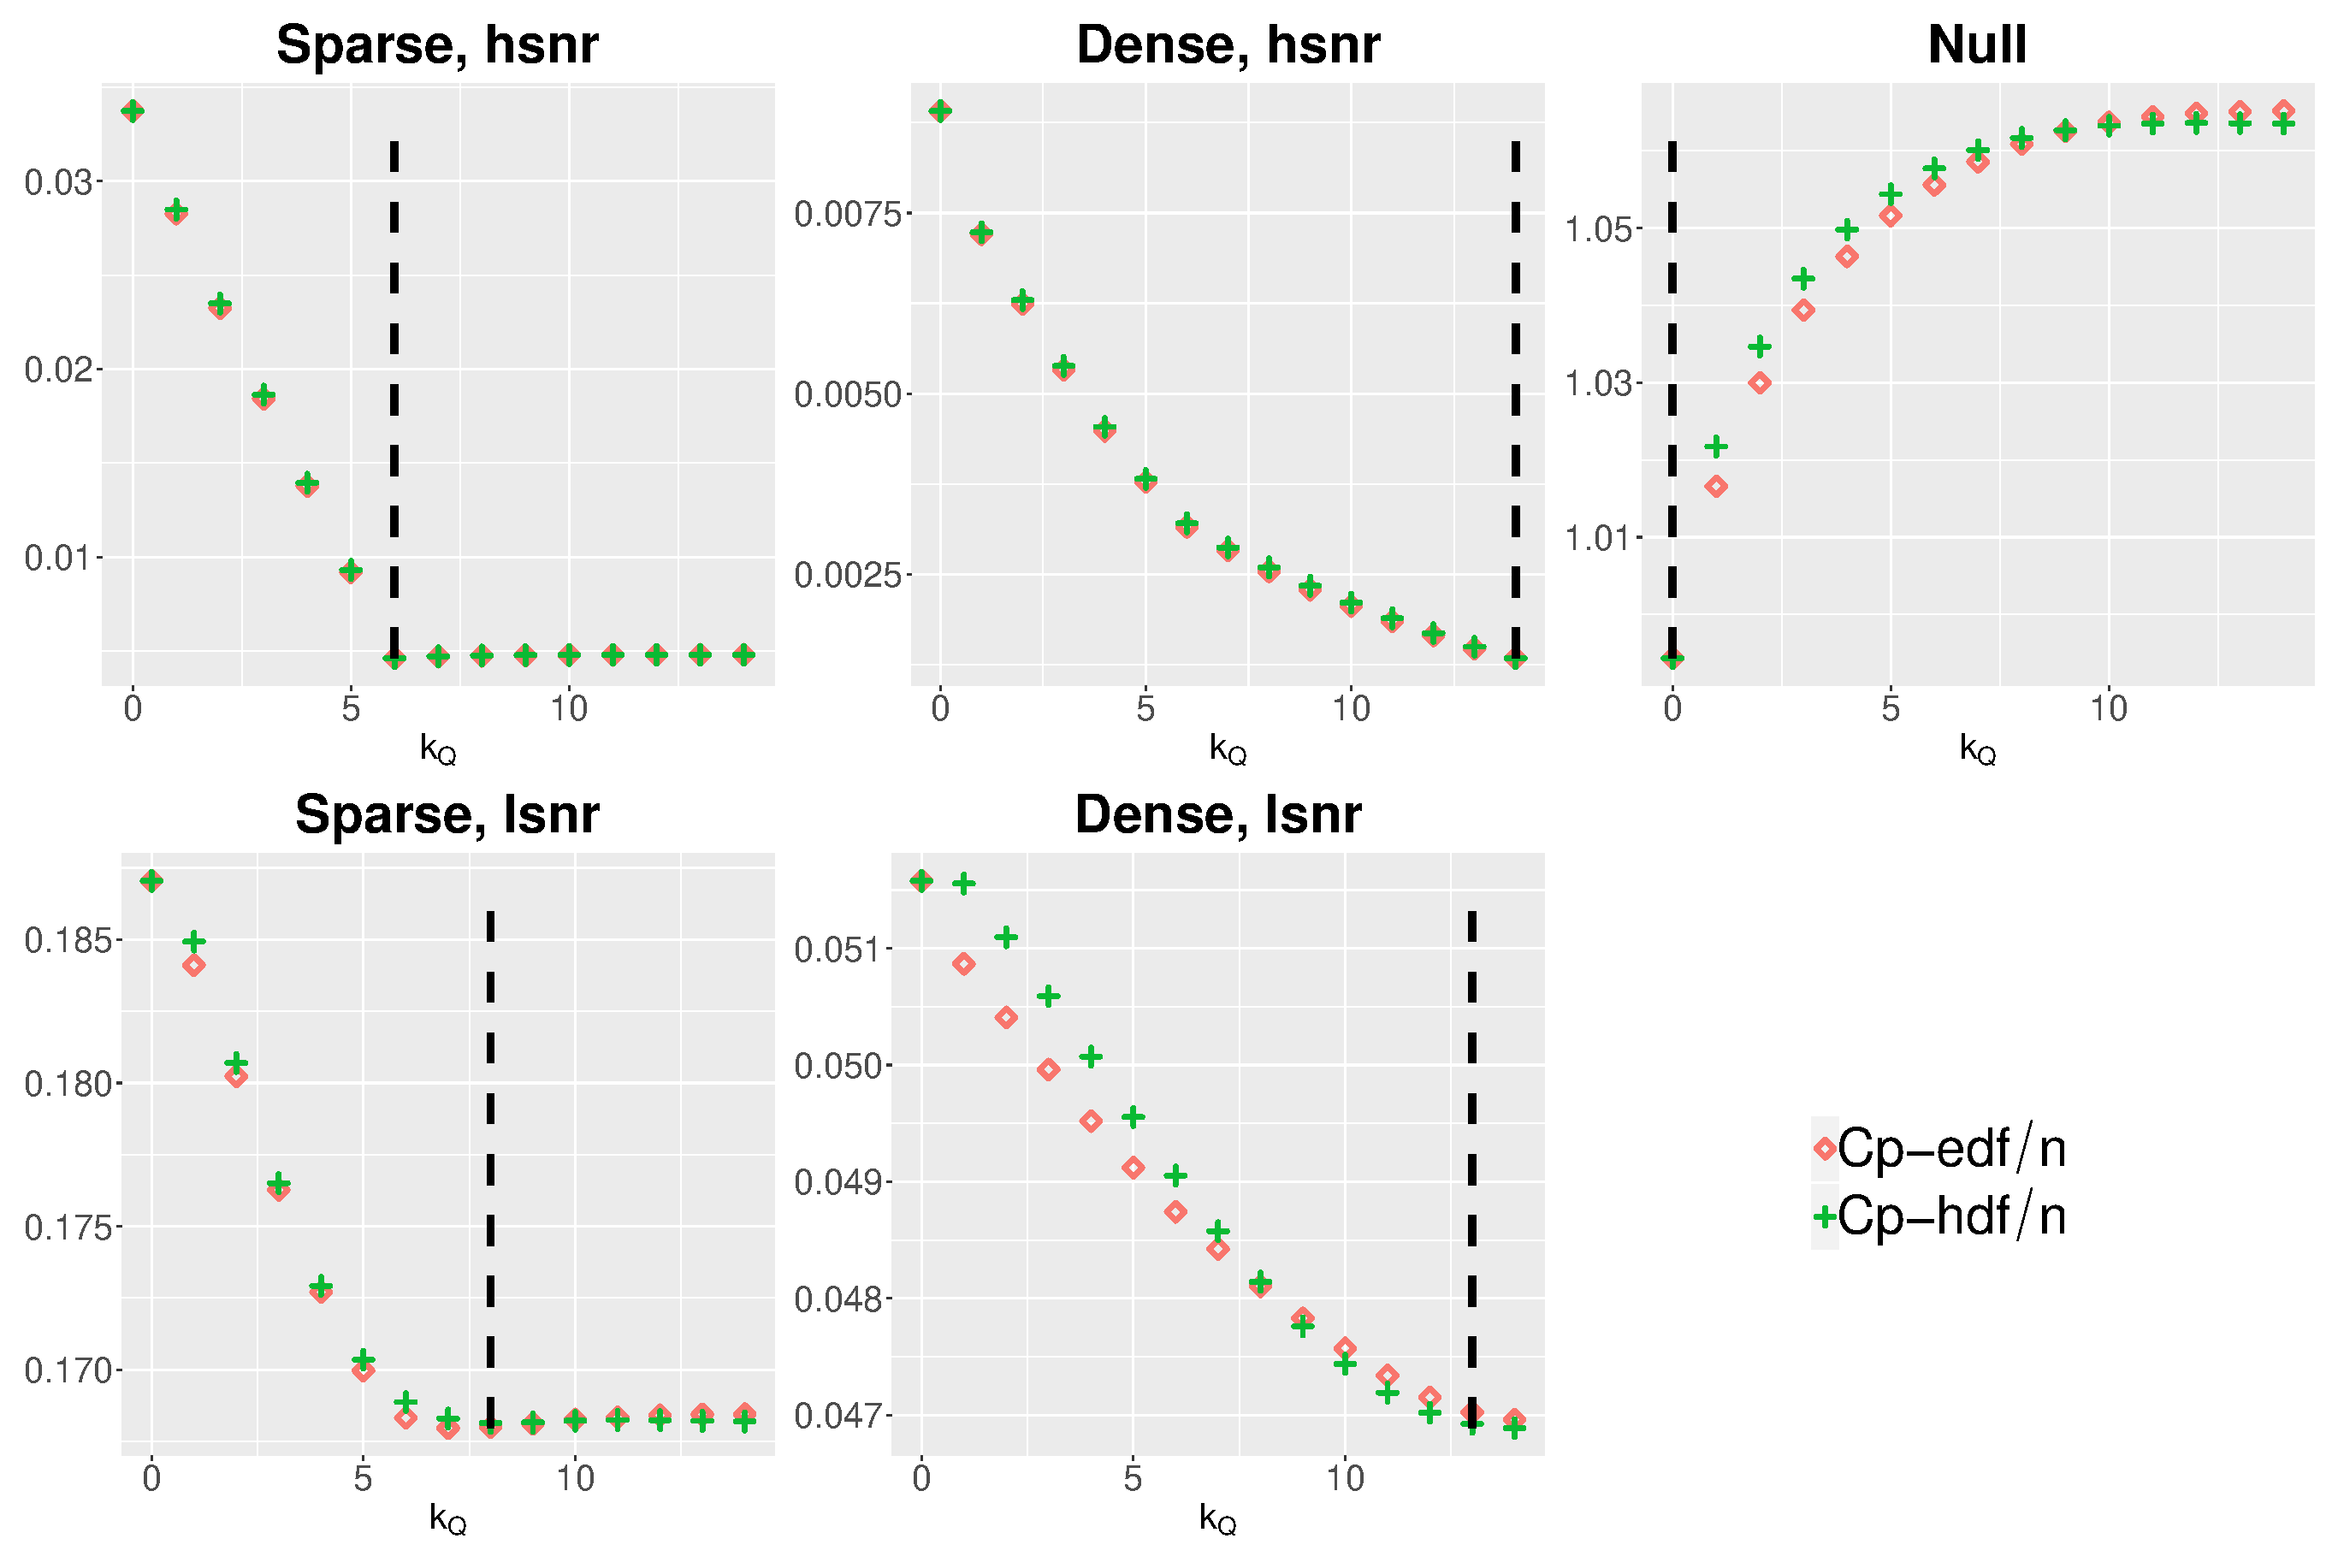
\includegraphics[width=0.9\textwidth]{figures/cp_edf_hdf_boss.eps}
	\caption{Averages of C$_p$-edf and C$_p$-hdf for BOSS over $1000$ replications. Here $X$ is general with $n=200$, $p=14$. Both criteria result in the same average of the selected subset size over the $1000$ replications (rounded to the nearest integer) as denoted by the dashed vertical lines. We assume knowledge of $\mu$ and $\sigma$.}
	\label{fig:boss_cp_edf_hdf}
\end{figure}


% {tab:lbs_bs}
% latex table generated in R 3.6.1 by xtable 1.8-4 package
% Sun Nov 10 00:24:03 2019
\begin{table}[ht]
\centering
\caption{The performance of BS and LBS. The selection rule for both methods is C$_p$-edf. We assume knowledge of $\mu$ and $\sigma$.} 
\label{tab:lbs_bs}
\scalebox{0.9}{
\begin{tabular}{|c|c|c|cc|cc|cc|}
  \toprule 
 \multicolumn{1}{|c}{} & \multicolumn{1}{c}{} &       & \multicolumn{2}{c|}{Orth-Sparse-Ex1} & \multicolumn{2}{c|}{Orth-Sparse-Ex2} & \multicolumn{2}{c|}{Orth-Dense} \\
 \cmidrule{4-9}\multicolumn{1}{|c}{} & \multicolumn{1}{c}{} &       & BS    & LBS   & BS    & LBS   & BS    & LBS  \\
 \midrule 
 \multicolumn{1}{|c}{} & \multicolumn{1}{c}{} &       & \multicolumn{6}{c|}{\% worse than the best possible BS} \\
 \midrule 
 \multirow{4}[4]{*}{n=200} & \multirow{2}[2]{*}{hsnr} & p=30 & 4 & 28 & 21 & 25 & 1 & 1 \\ 
   &  & p=180 & 1 & 43 & 12 & 25 & 7 & 10 \\ 
  \cmidrule{2-9} & \multirow{2}[2]{*}{lsnr} & p=30 & 20 & 26 & 21 & 30 & 15 & 16 \\ 
   &  & p=180 & 15 & 20 & 15 & 32 & 8 & 12 \\ 
  \midrule \multirow{4}[4]{*}{n=2000} & \multirow{2}[2]{*}{hsnr} & p=30 & 3 & 29 & 3 & 28 & 0 & 0 \\ 
   &  & p=180 & 0 & 42 & 0 & 41 & 6 & 9 \\ 
  \cmidrule{2-9} & \multirow{2}[2]{*}{lsnr} & p=30 & 3 & 28 & 7 & 25 & 2 & 2 \\ 
   &  & p=180 & 0 & 41 & 1 & 37 & 8 & 12 \\ 
   \midrule 
 \multicolumn{1}{|c}{} & \multicolumn{1}{c}{} &       & \multicolumn{6}{c|}{Relative efficiency} \\
 \midrule 
\multirow{4}[4]{*}{n=200} & \multirow{2}[2]{*}{hsnr} & p=30 & 1 & 0.81 & 1 & 0.96 & 1 & 1 \\ 
   &  & p=180 & 1 & 0.71 & 1 & 0.89 & 1 & 0.97 \\ 
  \cmidrule{2-9} & \multirow{2}[2]{*}{lsnr} & p=30 & 1 & 0.96 & 1 & 0.93 & 0.95 & 0.94 \\ 
   &  & p=180 & 1 & 0.96 & 1 & 0.87 & 1 & 0.95 \\ 
  \midrule \multirow{4}[4]{*}{n=2000} & \multirow{2}[2]{*}{hsnr} & p=30 & 1 & 0.8 & 1 & 0.81 & 1 & 1 \\ 
   &  & p=180 & 1 & 0.71 & 1 & 0.71 & 1 & 0.98 \\ 
  \cmidrule{2-9} & \multirow{2}[2]{*}{lsnr} & p=30 & 1 & 0.81 & 1 & 0.86 & 1 & 1 \\ 
   &  & p=180 & 1 & 0.71 & 1 & 0.74 & 1 & 0.97 \\ 
   \midrule 
 \multicolumn{1}{|c}{} & \multicolumn{1}{c}{} &       & \multicolumn{6}{c|}{Sparsistency (number of extra variables)} \\
 \midrule 
\multirow{4}[4]{*}{n=200} & \multirow{2}[2]{*}{hsnr} & p=30 & 6(0.1) & 6(0.7) & 4.8(0.4) & 5(0.9) & 30 & 29.9 \\ 
   &  & p=180 & 6(0) & 6(0.9) & 4.2(0) & 4.6(0.9) & 20.5 & 21.9 \\ 
  \cmidrule{2-9} & \multirow{2}[2]{*}{lsnr} & p=30 & 4.5(1.9) & 4.4(2.3) & 2.7(0.6) & 2.9(1.1) & 12.8 & 7.6 \\ 
   &  & p=180 & 1.9(0.5) & 2.3(1.4) & 1.9(0.3) & 2.2(1.2) & 0.8 & 2.7 \\ 
  \midrule \multirow{4}[4]{*}{n=2000} & \multirow{2}[2]{*}{hsnr} & p=30 & 6(0.1) & 6(0.7) & 6(0.1) & 6(0.7) & 30 & 30 \\ 
   &  & p=180 & 6(0) & 6(0.8) & 6(0) & 6(0.8) & 32.1 & 34.1 \\ 
  \cmidrule{2-9} & \multirow{2}[2]{*}{lsnr} & p=30 & 6(0.1) & 6(0.7) & 4.1(0.2) & 4.3(0.7) & 28.8 & 29.4 \\ 
   &  & p=180 & 6(0) & 6(0.8) & 4(0) & 4.1(0.8) & 13.9 & 15.9 \\ 
   \bottomrule 
\end{tabular}
}
\end{table}


\clearpage
\begin{figure}[!ht]
	\centering
	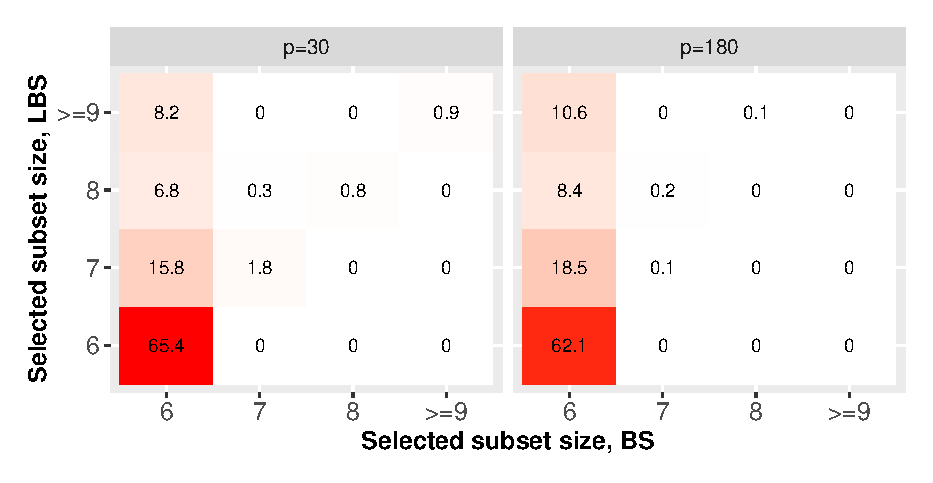
\includegraphics[width=0.9\textwidth]{figures/numvar_bs_lbs.eps}
	\caption{Frequency distributions (in $\%$) of the selected subset size  given by BS and LBS, based on $1000$ replications. The selection rule is C$_p$-edf. The true model is Orth-Sparse-Ex1 with $n=200$, $p_0=6$ and high SNR.}
	\label{fig:numvar_bs_lbs} 
\end{figure}


\iffalse
\begin{figure}[!ht]
	\centering
	\includegraphics[width=0.8\textwidth]{figures/lbs_bs_cp_eg.eps}
	\caption{C$_p$-edf at subset size $k$ for BS and LBS. The true model is Orth-Sparse-Ex1 with $n=200$, $p=180$, $p_0=6$ and high SNR. We assume knowledge of $\mu$ and $\sigma$.}
	\label{fig:lbs_bs_cp_eg} 
\end{figure}
\fi


\clearpage
\bibliographystyleonline{chicago}
\bibliographyonline{reference.bib}